\documentclass[24pt, a0paper, portrait, margin=5mm, innermargin=0mm,
               blockverticalspace=0mm, % space between blocks
               blocktitlewidthratio=0.6, colspace=10mm, 
               subcolspace=0mm]{tikzposter} 

% Change font     
\renewcommand{\familydefault}{\sfdefault}

% LATEX PACKAGES
% --------------
  
\usepackage{graphicx}  % package for inserting images, including .pdf
\usepackage{adjustbox} % package for cropping images
\usepackage{url} % package for url 
\usepackage{wrapfig}
\usepackage{lmodern} %mix italic and bold
\usepackage{hyperref}% for url
\usepackage{authblk}
\usepackage{graphicx} 
\usepackage{caption}
\usepackage{mwe}
\usepackage[absolute]{textpos}
\usepackage{selinput}
\usepackage{multicol}
\usepackage{tikz}
\usepackage{authblk} % improved author and affiliation design
\usepackage[none]{hyphenat} % avoid hyphenation

% \usepackage{anyfontsize} %increase overall font size
\SelectInputMappings{%
  Lcaron={Ľ}
}

\definecolor{amethyst}{rgb}{0.6, 0.4, 0.8}
\definecolor{babyblue}{rgb}{0.54, 0.81, 0.94}

% TITLE, AUTHORS, INSTITUTE
% -------------------------

\title{\textbf{\parbox{\linewidth}{\centering Methylation inheritance in three-spined sticklebacks (\textit{Gasterosteus aculeatus}) in response to parasite infection}}}

\author{\Large Alice~Balard\textsuperscript{1,*}, Kostas~Sagonas\textsuperscript{2}, Joshka~Kaufmann\textsuperscript{3}, Christophe~Eizaguirre\textsuperscript{1}}

\institute{\large \textsuperscript{1}School of Biological and Behavioural Sciences, Queen Mary University of London, UK; \textsuperscript{2}Faculty of Biosciences and Aquaculture, Nord University, Norway; \textsuperscript{1}University College Cork, Ireland \& Marine Institute, Newport, Ireland; \textsuperscript{*}Corresponding author: a.balard@qmul.ac.uk; Twitter: @alice\_balard; @EizaguirreLab}\vspace{-4ex}% reduce space


\titlegraphic{

\includegraphics[width=15cm]{fig/qm-logo-white.pdf}
}

\makeatletter
% improve affiliations: 1 line
\renewcommand\AB@affilsepx{, \protect\Affilfont}
%\renewcommand\AB@affilsepx{\quad\protect\Affilfont} % put affiliations into one line

\def\maketitle{\AB@maketitle}

% increase tikzfigure caption  font size
\renewenvironment{tikzfigure}[1][]{
  \def \rememberparameter{#1}
  \vspace{10pt}
  \refstepcounter{figurecounter}
  \begin{center}
  }{
    \ifx\rememberparameter\@empty
    \else %nothing
    \\[10pt]
    {\Large Fig.~\thefigurecounter: \rememberparameter}
    \fi
  \end{center}
}

\makeatother

% THEME SETTING
% -------------
\usetheme{Simple}
\colorlet{titlebgcolor}{babyblue}
\colorlet{titlefgcolor}{black}
\colorlet{blocktitlebgcolor}{gray}
\colorlet{blocktitlefgcolor}{gray}

\colorlet{blocktitlebodycolor}{red}

% HEAD
% ----

\begin{document}
\maketitle[linewidth = 1mm]

% add fish picture next to title block
\node[anchor=west] at (TP@title.west) {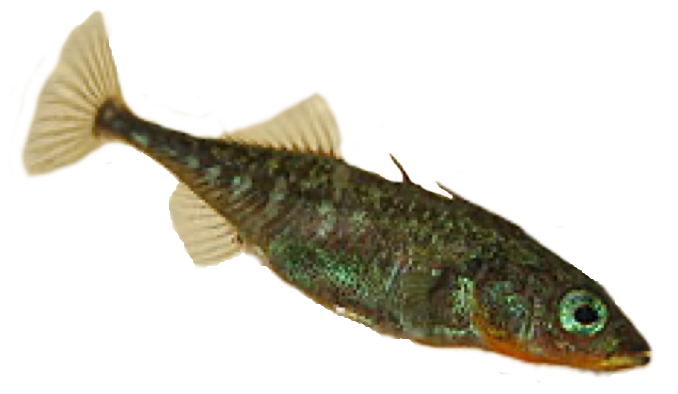
\includegraphics[width=13cm]{fig/stickpic.png}};

% Context
% ----
\block{Background}
{\Large Parasite pressure influences the evolution of resistance and tolerance mechanisms in their hosts. In a two-generation infection experiment of three-spined stickleback (\textit{Gasterosteus aculeatus}) by the nematode \textit{Camallanus lacustris}, paternal infection, despite imposing a \textbf{cost} on the next generation, also presented \textbf{benefits for offspring’s tolerance}\textsuperscript{1}. The methylation pattern was shown to differ between infected and control parents\textsuperscript{2}.\\ \textbf{Aim: Understanding the role and mechanisms of phenotypic plasticity within and across generations, focusing on DNA methylation. Which of the DNA methylations linked to parasite infection can be transmitted to the next generation?}
}	


% MATANDMET
% ----

\begin{columns}

  \column{0.4} \block{}{
  
   \begin{tikzfigure}[Experimental design]
               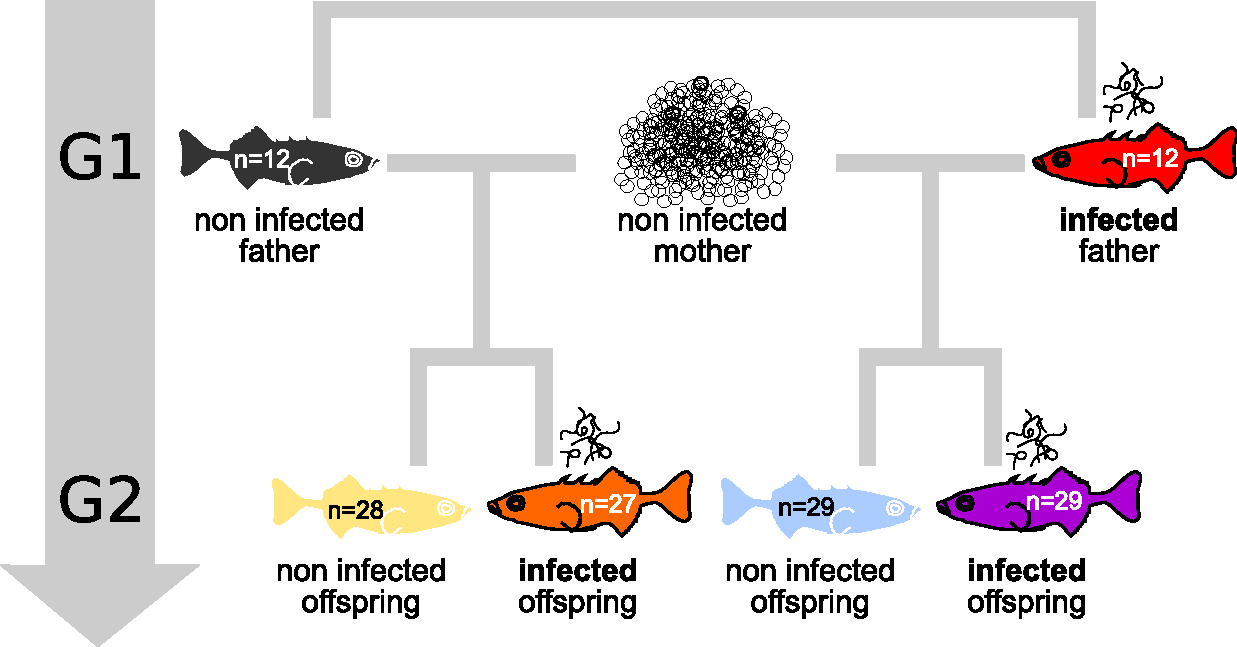
\includegraphics[scale=1.3]{fig/designExpe.pdf}
    \end{tikzfigure}
    }
    
  \column{0.6} \block{Material \& methods}{\Large
    \begin{enumerate}
      \item \textbf{Experimental design:} \textbf{G0 generation} from natural lake population -> \textbf{G1 generation} of full-sib fish families. In vitro mating of G1 males and G1 gravid female from another family serving as egg donor, repeated in brother pairs within each male family (1 from G1 “treatment” group and 1 from G1 “control” group) -> \textbf{G2}. Infection of G1 \& G2 with \textit{C. lacustris} larvae through copepod ingestion (Fig.1)
      \item \textbf{Data processing:} Methylome sequencing: Reduced Representation Bisulfite Sequencing (RRBS) single-end reads of 100bp long, Illumina HiSeq 2500. Alignment on a European gynogen genome\textsuperscript{3} and methylation call by BSBolt. Downstream analyses by Methylkit.
    \end{enumerate}
  }
  
\end{columns}

% Results: 
% -------

\block{Preliminary results}

% first row: the figures
\begin{columns}\column{0.25}

\block{}{ \vspace{-5ex}% reduce space between block and previous block
\Large \centering \begin{tikzfigure}[Paternal treatment effect on offspring body condition] 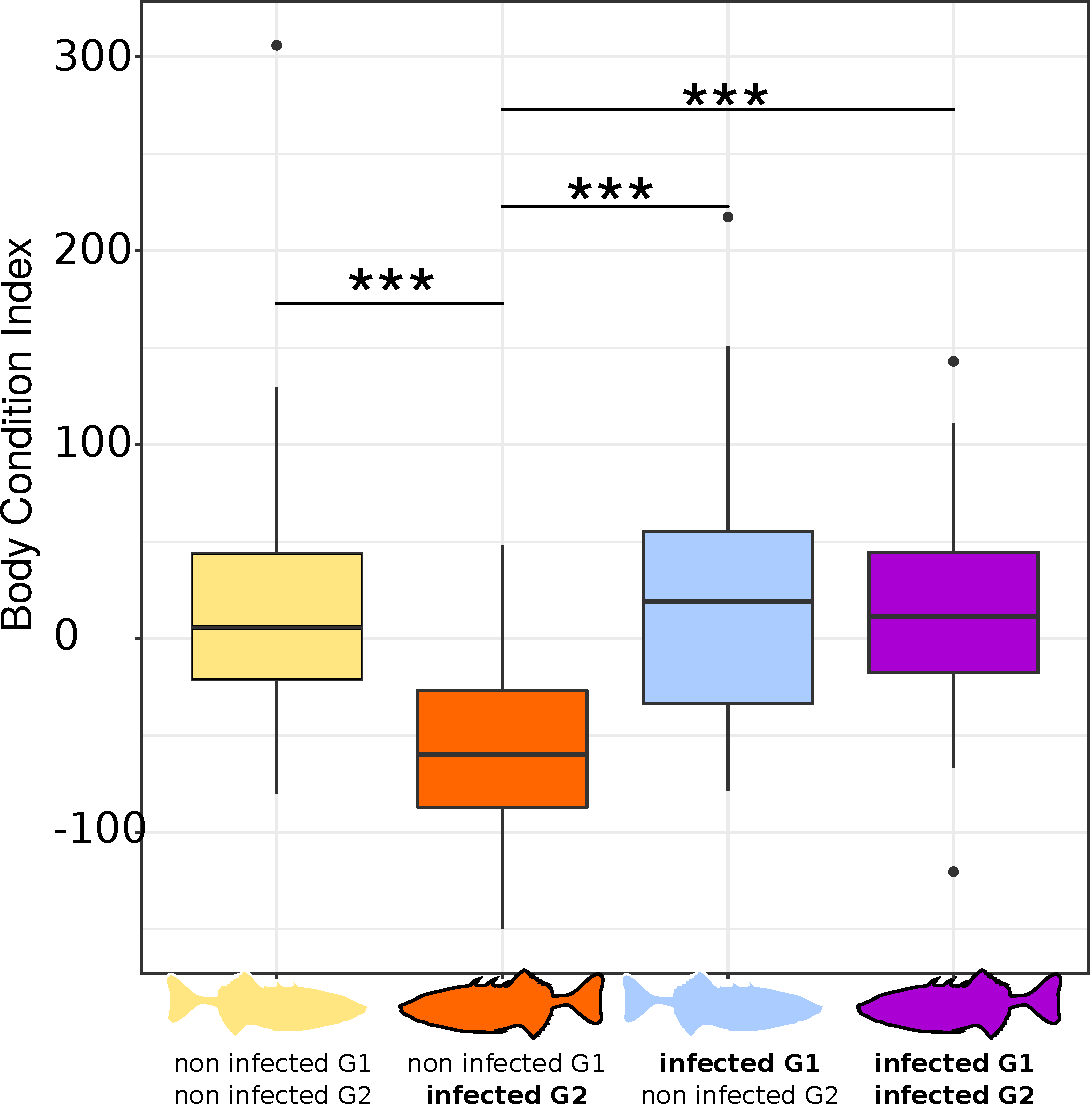
\includegraphics[scale = 1.1]{fig/BCIoffspring_pretty.pdf}
  \end{tikzfigure}
}

\column{0.75}

\block{}{ \vspace{-5ex}% reduce space between block and previous block
\Large \centering \begin{tikzfigure}[Hierarchical clustering of individual fish CpG methylation] 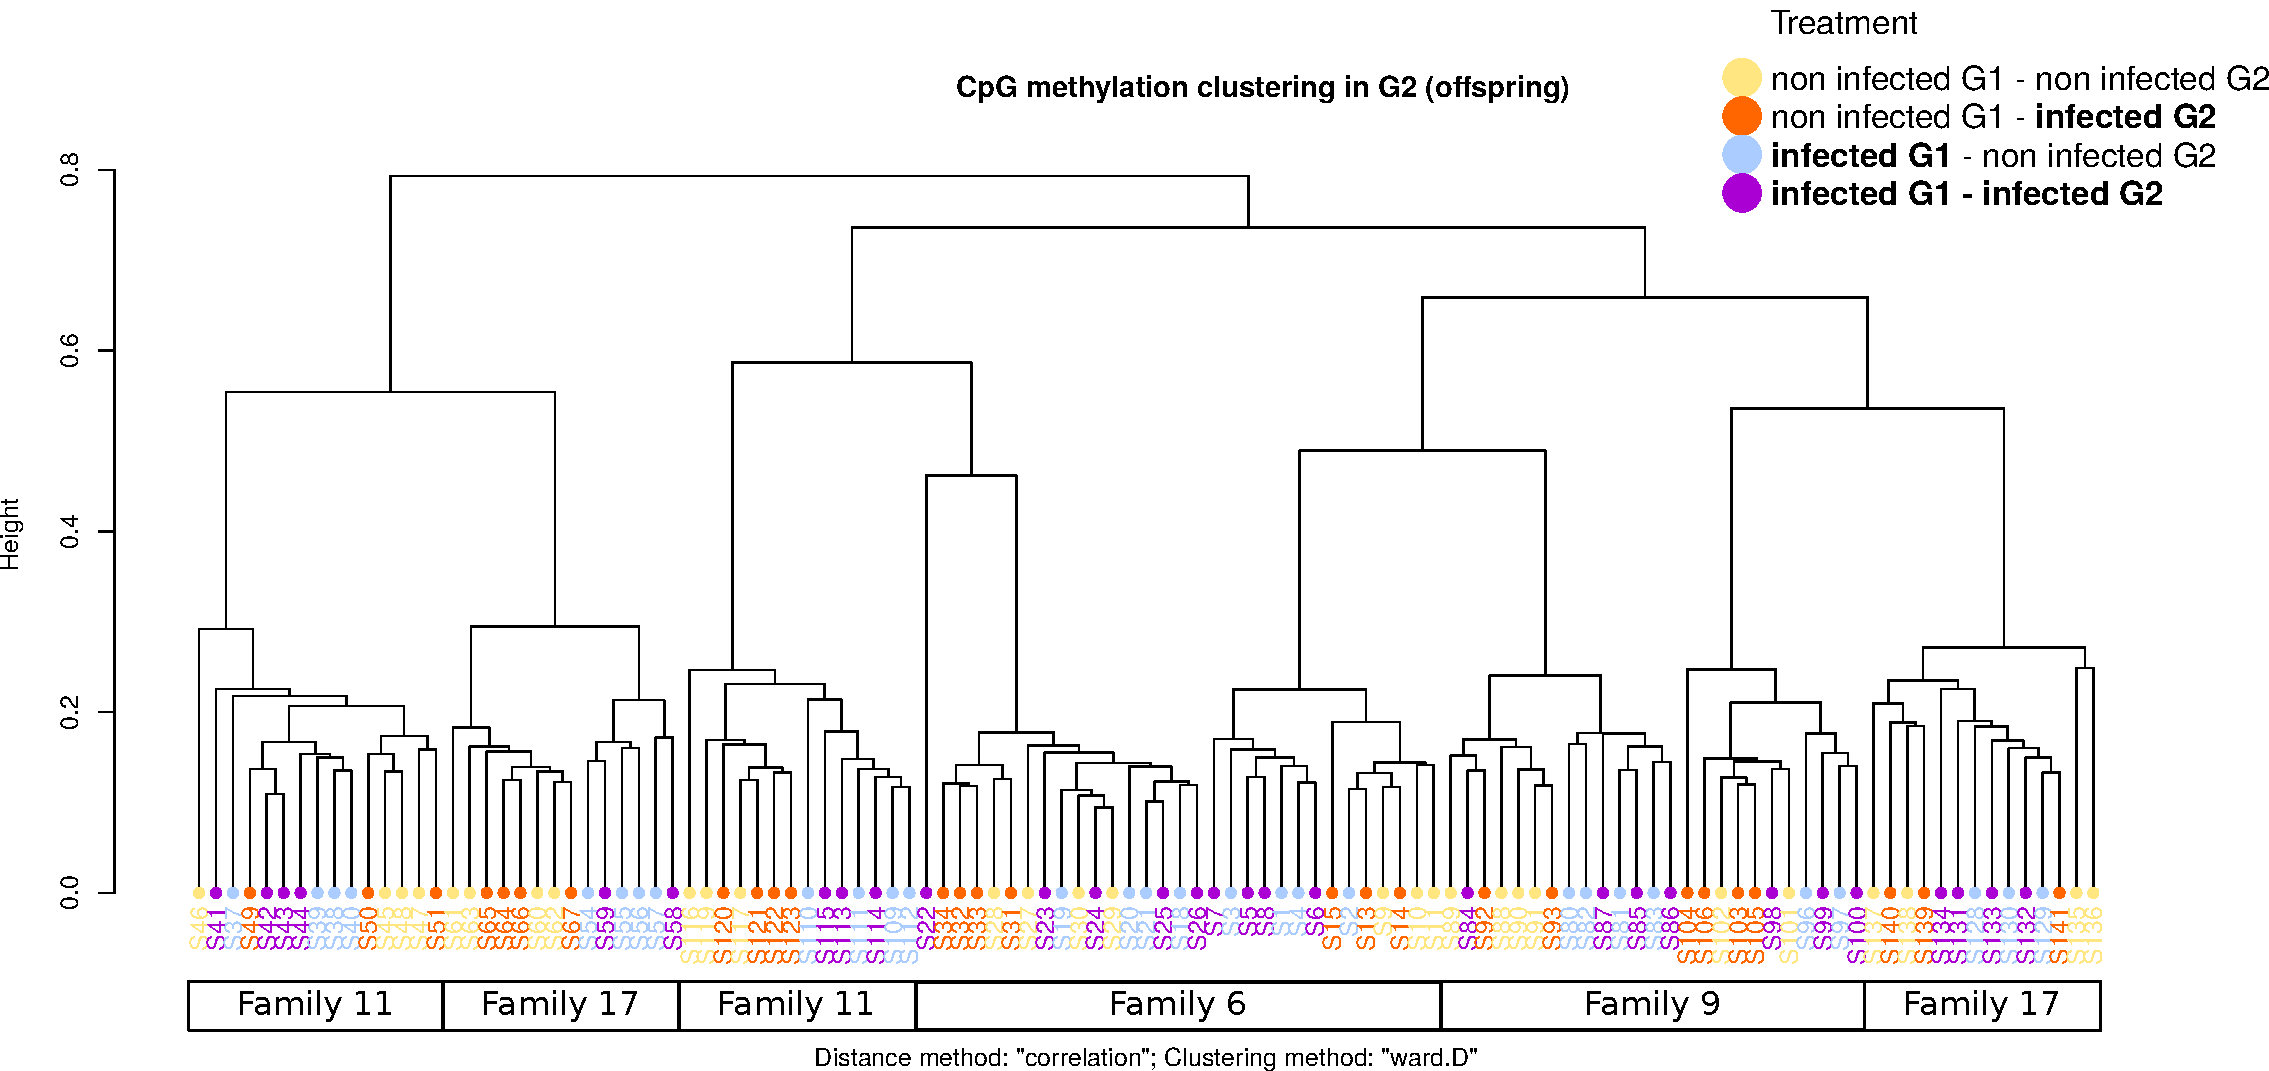
\includegraphics[scale = 1.3]{fig/clusterALLCpG_offsprings_pretty.pdf}
  \end{tikzfigure}
}
\end{columns}

% second row: text
\block{}{
\Large \textbf{Paternal treatment affects body condition} (BC): infected offspring from non infected father show a decrease in BC after infection; this drop is absent in infected fish from infected father (Fig.2). This confirms on our data subset the results of Kaufmann et al.\textsuperscript{1} 
}

\block{}{
\Large\textbf{Offspring methylomes cluster by family and paternal treatment}: within family subgroups, the paternal treatments seems to play a stronger role in clustering than the treatment of offspring itself (Fig.3).
}

% PERSPECTIVE
% ----------
\block{Perspective}{\Large
\begin{enumerate}

  \item Compare Differentially Methylated Sites (DMS), hypo and hypermethylation, between offspring groups:

    \begin{enumerate}
      \item \textbf{Tests of parental effect:} \newline comparison of (\colorbox{yellow}{G1 non infected-G2 non infected} vs \colorbox{babyblue}{G1 infected-G2 non infected}), and (\colorbox{orange}{G1 non infected-G2 infected} vs \colorbox{amethyst}{G1 infected-G2 infected})
      \item \textbf{Tests of offspring exposure:} \newline comparison of (\colorbox{yellow}{G1 non infected-G2 non infected} vs \colorbox{orange}{G1 non infected-G2 infected}) and (\colorbox{babyblue}{G1 infected-G2 non infected} vs \colorbox{amethyst}{G1 infected-G2 infected})
    \end{enumerate}
  
  \item Identification of genes and genes networks (method: WGCNA) involved

\end{enumerate}

}

\begin{columns} 
  \column{0.8} 
  
% REFERENCES
% ----------
  \block{References}{
\textsuperscript{1}Kaufmann, J., Lenz, T. L., Milinski, M., \& Eizaguirre, C. (2014). Experimental parasite infection reveals costs and benefits of paternal effects. Ecology Letters; \textsuperscript{2}Sagonas, K., Meyer, B. S., Kaufmann, J., Lenz, T. L., Häsler, R., \& Eizaguirre, C. (2020). Experimental parasite infection causes genome-wide changes in DNA methylation. Molecular Biology and Evolution; \textsuperscript{3}Thornburn et al., in prep.
  }

% FUNDING
% ----------
\column{.2}
   \block[]{}{\LARGE \centering \vspace{-4ex}
    \textbf{Funding}
    \begin{tikzfigure}[]
    
\includegraphics[scale=3.5]{fig/logo--en.pdf}
   \end{tikzfigure}}
   
\end{columns}

% ----------------
\end{document}
\endinput
%%
%% End of file 
